\documentclass[11pt,a4paper,notitlepage]{report} % notitlepage doesnt reset pagenumber on abstract
\usepackage[portuguese]{babel}
\usepackage[latin1,utf8]{inputenc} %utf8 for linux
\usepackage[T1]{fontenc}
\usepackage{hyperref}
%\usepackage[a4paper, pdftex, bookmarks, colorlinks, linkcolor=black, urlcolor=blue]{hyperref} %por linkcolor=cor para ter os links com cor.
\usepackage[a4paper,left=3cm,right=2.5cm,top=3cm,bottom=2.5cm]{geometry}
%\usepackage[margin=10pt,font=small,labelfont=bf]{caption}
%\usepackage{graphicx}
\usepackage{float} % for floating objects
%\usepackage{multirow}
\usepackage{array}
\usepackage{amsfonts}
\usepackage{amsmath}
\usepackage{mathtools}
%\usepackage[table]{xcolor}
\usepackage[section]{placeins} % para os floats nao ultraparassem a section em que sao criados
%\usepackage[portuguese]{nomencl} % para a lista de nomenclaturas
%\makenomenclature
%\usepackage[toc,page]{appendix}
\usepackage{algpseudocode} % for algorithms
\usepackage{algorithm} % for algorithms
\usepackage[titletoc]{appendix} % as seen here: http://stackoverflow.com/questions/5690679/add-appendix-before-a-in-thesis-toc
%\usepackage[nottoc]{tocbibind} % para meter a bibliografia no toc
\usepackage{enumerate} % para o enumerate a), b)
\usepackage{listings}
\usepackage[margin=10pt,font=small,labelfont=bf]{caption}
\usepackage{color}
\usepackage{todonotes} % Mark­ing things to do in a LATEX doc­u­ment
\usepackage{hyperref}
\usepackage{datetime} % pre-defined dates
\usepackage{alltt} % formatted verbatim
\usepackage{comment}
%
\newenvironment{definition}[1][Definição]{\begin{trivlist}
\item[\hskip \labelsep {\bfseries #1}]}{\end{trivlist}}
\newenvironment{example}[1][Exemplo]{\begin{trivlist}
\item[\hskip \labelsep {\bfseries #1}]}{\end{trivlist}}
\setlength\parindent{0pt} % Removes all indentation from paragraphs - comment this line for an assignment with lots of text
%
%%%%%%%%%%%%%%%%%%%%%%%%%%%%%
% new commands
%%%%%%%%%%%%%%%%%%%%%%%%%%%%%
\newcommand{\HRule}{\rule{\linewidth}{0.5mm}} % para a capa
\newcommand{\sage}{\texttt{Sage}}
\newcommand{\RingLPN}{\textsf{Ring-LPN}}
\newcommand{\RingLPNR}{\textsf{Ring-LPN}$\mathsf{^R}$}
\newcommand{\RingLPNRtau}{\textsf{Ring-LPN}$\mathsf{^R_\tau}$}
%
%
% mudar algorithm para algoritmo
\floatname{algorithm}{Algoritmo}
\renewcommand{\algorithmicrequire}{\textbf{Input:}}
\renewcommand{\algorithmicensure}{\textbf{Output:}}
% mudar appendices para anexos
\renewcommand{\appendixtocname}{Apêndices}
\renewcommand{\appendixpagename}{Apêndices}
% floating algorithms
\newfloat{algorithm}{t}{lop}
% mudar list of nomenclatures para palavras chave
%\renewcommand{\nomname}{Palavras Chave}
%
% listings
\definecolor{dkgreen}{rgb}{0,0.6,0}
\definecolor{gray}{rgb}{0.5,0.5,0.5}
\definecolor{mauve}{rgb}{0.58,0,0.82}
\renewcommand{\lstlistingname}{Código}
\lstdefinestyle{sage}{
  frame=tb,
  language=Python,
  tabsize=2,
  breaklines=true,
  breakatwhitespace=true,
  basicstyle={\footnotesize\ttfamily},
  aboveskip=3mm,
  belowskip=3mm,
  numberstyle=\tiny\color{gray},
  keywordstyle=\color{blue},
  commentstyle=\color{dkgreen},
  stringstyle=\color{mauve},
  showstringspaces=false,
  captionpos=t,
  %morecomment=[is]{\#}{ } % could be used to hide comments
}
\lstdefinestyle{C}{
  frame=tb,
  language=C,
  tabsize=2,
  breaklines=true,
  breakatwhitespace=true,
  basicstyle={\footnotesize\ttfamily},
  aboveskip=3mm,
  belowskip=3mm,
  numberstyle=\tiny\color{gray},
  keywordstyle=\color{blue},
  commentstyle=\color{dkgreen},
  stringstyle=\color{mauve},
  showstringspaces=false,
  captionpos=t,
  %morecomment=[is]{\#}{ } % could be used to hide comments
}
% \include includes the file in a new page
% \input include the file in the current page
% \chapter[short description]{long description}
% use \and when using more than one author
% to use bibtex: \cite{citation_name}
%
%
\begin{document}
\pagenumbering{roman}
\begin{titlepage}

\begin{center}

% Upper part of the page

\includegraphics[width=0.25\textwidth]{img/um-eng}\\[1cm]

\textsc{\LARGE Universidade do Minho\\Departamento de Informática}\\[1cm]

\textsc{\Large Criptografia e Segurança dos Sistemas de Informação}\\[0.5cm]
\textsc{\Large Projecto Integrador II\\2012/2013}\\[0.25cm]


% Title
\HRule \\[0.4cm]
{ \huge \bfseries Post quantum authentication}
\HRule \\[1.5cm]
%
% Author and supervisor
\begin{minipage}[t]{0.4\textwidth}
\begin{flushleft} \large
pg22797 Milton \textsc{Nunes}\\
%[1.5cm]
pg22815 Nuno \textsc{Carvalho}\\
%[1.5cm]
\end{flushleft}
\end{minipage}
\begin{minipage}[t]{0.4\textwidth}
\begin{flushright} \large
\textbf{Supervisor:}\\
Prof. Manuel Bernardo \textsc{Barbosa}
\end{flushright}
\end{minipage}

\vfill

% Bottom of the page

{\large \today}

\end{center}
%\newpage
%\thispagestyle{empty} % no pagenumber on this page
%\begin{center}
%  \vspace*{\fill}
%  \begin{tabular}{m{3cm} m{0.5cm}}
%%  %\begin{tabular}{c}
%%    % demasiado escaxe LOL
%%    %\includegraphics[width=0.55\textwidth]{../img/grupo/escaxe}\\
%%    %(esq para dir) Milton Nunes, Nuno Carvalho, Rafael Remondes\\
%    Milton Nunes & 
\includegraphics[width=0.15\textwidth]{img/grupo/milton}\\ \\
%    Nuno Carvalho & 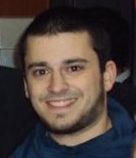
\includegraphics[width=0.15\textwidth]{img/grupo/teddy}\\ \\
%  \end{tabular}
%  \vspace*{\fill}
%\end{center}
\end{titlepage}

%
%\maketitle
\newpage
%
% the abstract
\begin{abstract}
\thispagestyle{plain} % pagenumber on abstract page
Com o eventual aparecimento dos computadores quânticos, os esquemas de assinaturas baseados no problema da factorização ou do logaritmo discreto tornar-se-ão inúteis. Dado que a maioria dos esquemas baseiam-se na teoria de número, acredita-se que com esse eventual aparecimento estes problemas deixarão de ser difíceis e por isso sem utilidade na criptografia. Posto isto, tornou-se imperativo procurar esquemas de assinaturas digitais que se apresentassem como alternativas viáveis. Esta procura levou a que se chegassem a esquemas baseados em reticulados, que se revelaram uma alternativa válida ao problema que se pretendia resolver e que proporcionaram avanços significativos em várias áreas da criptografia.\\

Este Projecto Integrador pretende abordar e explorar a aplicabilidade de esquemas criptográficos de autenticação de mensagens baseados em reticulados. Assim, neste relatório será apresentado todo o trabalho de análise e estudo efectuado sobre as duas publicações sugeridas \cite{lapin,lattice_sig}. Do estudo resultaram dois protótipos em \sage: um do protocolo Lapin \cite{lapin} e outro do protocolo de assinatura baseado em reticulados \cite{lattice_sig}. Além disso será apresentada a implementação em \textsf{C} do protocolo Lapin.
\end{abstract}
%
%
%
%
%%% Antigo
\newpage
%
%\input{nomenclature}
%\printnomenclature
%\newpage
%table of contents
\tableofcontents
\newpage
%
\pagenumbering{arabic}
\chapter{Introdução}
\section{Objectivos}
Numa primeira fase o objectivo pretendido consistiu em estudar um novo protocolo autenticação de forma a poder desenvolver um pequeno protótipo  em \sage, uma ferramenta com a qual estávamos familiarizados dado que foi utilizada no primeiro Projecto Integrador. Nesta fase foi também possível efectuar um estudo das operações aritméticas sobre polinómios mais eficientes, apenas com o uso de operações binárias.\\
Neste última fase era pretendido que fosse feita a implementação do protocolo estudado na primeira fase num linguagem mais eficiente. Foram consideradas para a implementação do protocolo as linguagens \textsf{C}, \textsf{C++} e \textsf{Java}. Apesar de a linguagem em que nos sentimos mais confortáveis ser \textsf{Java}, considerámos que esta é a menos eficiente e a menos indicada para dispositivos \textit{low-cost}, portanto optámos por \textsf{C} (nunca utilizámos \textsf{C++} e não nos pareceu que oferecesse vantagens em relação ao \textsf{C}).\\
O resto do presente documento apresenta todo o estudo efectuado sobre as publicações, os protótipos desenvolvidos e ainda a implementação do protocolo de autenticação Lapin.\\
%%%%%%%%%%%%%%%%%%%%%%%%%%%%%%%%%%%%%5
\section{Computação quântica}
A possibilidade do aparecimento de computadores quânticos é um tema sensível e que gera muitas expectativas no seio da comunidade criptográfica. Isto deve-se ao facto de se acreditar que esta possibilidade deverá resolver determinados problemas usados em criptografia que se julgam difíceis, o que tornará vários esquemas inseguros.\\
Vários esquemas são baseados na dificuldade de problemas como a factorização de inteiros ou logaritmo discreto. A existência de computadores quânticos resolveria de forma eficiente estes problemas e assim inviabilizaria a utilização de algoritmos como o \textsf{RSA}. Isto afectaria vários sistemas cuja segurança é garantida pelo seu uso. Posto isto surgiu a necessidade de se encontrar soluções alternativas que não seja afectadas pela existência da computação quântica. Esta nova linha de investigação, cuja incidência sobre esquemas baseados em reticulados é bastante acentuado, tem conseguido resultados extremamente positivos, contudo é ainda prematuro garantir a sua aplicabilidade.
\section{Protocolo de autenticação}
Um protocolo de autenticação tem como objectivo a autenticação de duas entidades que pretendem efectuar uma comunicação segura. São protocolos de chave privada em que um \textit{prover} $\mathcal{P}$ autentica-se perante um \textit{verifier} $\mathcal{V}$.\\
Uma das famílias de protocolos de autenticação existente é o \textit{Challenge-Response}, que consiste num protocolo em que uma parte gera um \textit{challenge} que envia à outra parte, sendo que esta envia uma resposta que caso seja válida a autentica perante a primeira. Um exemplo trivial desta família de protocolos é o processo de autenticação de password, em que o challenge é o pedido de inserção da password correcta, sendo que caso esta seja válida a autenticação é alcançada.\\

\section{Protocolo de assinaturas}
Protocolos de assinaturas pretendem garantir que a autenticidade de uma mensagem. Através do uso destes protocolos o receptor tem a garantia de que quem enviou a mensagem é alguém por ele conhecido, este não pode negar esse envio, e ainda que a mensagem não foi alterada durante a comunicação. Ou seja, garante autenticação, não-repúdio e integridade da mensagem, respectivamente.\\
Os esquemas de assinaturas consistem tipicamente em três algoritmos: geração de chaves que gera o par de chaves, o algoritmo de assinatura que recebe a chave privada e a mensagem e gera a assinatura, e o algoritmo de verificação que recebe a mensagem, a assinatura e a chave pública e verifica se a assinatura é valida ou não.\\

No âmbito dos protocolos baseados em reticulados, já existem alguns esquemas criptográficos seguros e com aplicação prática, mas poucos esquemas de assinaturas seguros e com aplicação prática.
%%% Lapin
\chapter{Lapin}
%%%%%%%%%%%%%%
% Descricao
%%%%%%%%%%%%%%
%\section{Descrição}
O protocolo de autenticação Lapin apresentado em \cite{lapin} é baseado no problema \RingLPN\ (\textit{Ring variant of the Learning Parity with Noise}). Este protocolo, constituído por apenas dois \textit{rounds} é seguro contra ataques activos e tem uma complexidade de comunicação bastante pequena, pelo que é indicado para dispositivos \textit{low-cost} ou em cenários onde os recursos são limitados.\\
Em comparação com outros protocolos, que fazem uso de cifras por blocos como por exemplo o AES, o Lapin mostra-se como uma boa alternativa. Em casos onde se possuam algumas centenas de \textit{bytes} de memória não-volátil, onde se poderão guardar alguns resultados pré-computados, o protocolo apenas é apenas duas vezes mais lento que o AES, mas em compensação, tem cerca de dez vezes menos código do que o AES.\\
%%%%%%%%%%%%%%
% Definições
%%%%%%%%%%%%%%
\section{Definições}
%%%%%%%%%%%%%%%
% Polinomios
%%%%%%%%%%%%%%%
\subsection{Polinómios}
O protocolo baseia-se essencialmente em operações sobre polinómios binários, ou seja, polinómios em $\mathbb{F}_2[x]$. Todos os polinómios do protocolo pertencem ao anel $\mathbb{F}_2[x]/f(x)$, sendo que um elemento deste anel tem grau máximo $deg(f)-1$. No âmbito deste projecto, serão considerados dois anéis $\mathsf{R} = \mathbb{F}_2[x]/f(x)$: um anel em que $f(x)$ é irredutível e outro em que $f(x)$ é factorizável em $m$ polinómios distintos.
%Denota-se por $\widehat{a}$ a representação CRT (Teorema Chinês dos Restos) do polinómio $a$ em relação aos $m$ factores do $f(x)$ factorizável, ou seja, $\widehat{a} = (a \bmod{f_1}, \dotsc, a \bmod{f_m})$\\ \todo{se nao se falar mais disto no relatorio, nao vale a pena ter isto aqui..}
%%%%%%%%%%%%%%%%%%%%%%%%
% Distributions
%%%%%%%%%%%%%%%%%%%%%%%%
\subsection{Distribuições}
Uma distribuição $\mathcal{D}$ sobre determinado domínio representa-se sob a forma de $r \longleftarrow_{\$} \mathcal{D}$, sendo $r$ o valor gerado de acordo com a distribuição $\mathcal{D}$. Denomina-se uma distribuição uniforme sobre o domínio $Y$ como $\mathcal{U}(Y)$. Seja a distribuição de \textsf{Bernoulli},  $\textsf{Ber}_{\tau}$ sobre $\mathbb{F}_2$ com o parâmetro $\tau \in\ ]0,1/2[$. Para um anel polinomial $\mathsf{R} = \mathbb{F}_2[x]/f(x)$, a distribuição $\textsf{Ber}_{\tau}^\mathsf{R}$ denota a distribuição sobre polinómios de $\mathsf{R}$, para os quais os coeficientes são determinados independentemente de $\textsf{Ber}_{\tau}$.% Para um anel $\mathsf{R}$ e um polinómio $s \in \mathsf{R}$, representa-se $\Lambda_{\tau}^{\mathsf{R},s}$ como uma distribuição sobre $\mathsf{R} \times \mathsf{R}$ sendo as amostragens obtidas através dos polinómios $r \longleftarrow_{\$} \mathcal{U}(\mathsf{R)}$ e $e \longleftarrow_{\$} \mathsf{Ber}_{\tau}^\mathsf{R}$, cujo resultado é o seguinte \textit{output}: $(r, rs+e)$. \todo{Isto tb nao parece ser mais usado no resto do relatz}
%%%%%%%%%%%%%%%%
% RingLPN e LPN
%%%%%%%%%%%%%%%%
\subsection{\textit{Ring Learning Parity with Noise} (\RingLPN) e \textit{Learning Parity with Noise} (\textsf{LPN})}
A segurança do protocolo depende problema do \textsf{Ring-LPN} que se trata de uma expansão do problema \textsf{LPN} para anéis. Este problema pode também ser visto como uma instanciação particular de um outro problema com grande ligação aos reticulados, o \textsf{Ring-LWE} (\textit{Learning with Errors over Rings}).\\
A diferença entre os dois problemas reside na diferença entre dois possíveis oráculos. O primeiro oráculo gera aleatoriamente um vector secreto $s \in \mathbb{F}_2^n$ que é usado produzir a resposta. No problema \textsf{LPN}, cada chamada do oráculo produz, de forma uniforme, uma matriz aleatória $A \in \mathbb{F}_2^{n \times n}$ e um vector $As + e = t \in \mathbb{F}_2^n$, onde $e$ é um vector de $\mathbb{F}_2^n$ em que cada entrada é um valor aleatório gerado independentemente pela distribuição de \textit{Bernoulli} com a probabilidade de 1 usando o parâmetro público $\tau$ entre $0$ e $1 \setminus 2$. O segundo oráculo gera uma matriz $A \in \mathbb{F}_2^{n \times n}$ aleatória de forma uniforme e um vector aleatório $t \in \mathbb{F}_2^n$ de forma igualmente uniforme.\\
A diferença entre o \textsf{LPN} e o \textsf{Ring-LPN} está na geração da matriz $A$, em ambos os oráculos. Enquanto no problema \textsf{LPN} todas as entradas são geradas de forma uniforme e independente, no problema \textsf{Ring-LPN} apenas a primeira coluna é gerada dessa forma em $\mathbb{F}_2^n$, sendo que as restantes colunas dependem da primeira e do anel subjacente $\mathsf{R} = \mathbb{F}_2[x]/f(x)$. De assinalar ainda que a suposição $\textsf{Ring-LPN}^\mathsf{R}$ indica que é difícil distinguir entre os \textit{outputs} dos dois oráculos.\\
O problema \textsf{LPN} é bastante usado em criptografia como uma suposição difícil, ao contrário do \textsf{Ring-LPN}. Contudo, uma publicação recente demonstra que o problema \textsf{Ring-LWE} é tão difícil quanto resolver quanto o pior caso de um pequeno vector de reticulados. Por sua vez, o 
\textsf{Ring-LPN} é bastante semelhante ao problema \textsf{Ring-LWE}.
%%%%%%%%%%%%%%%%%%%
% Protocolo
%%%%%%%%%%%%%%%%%%%
\section{Protocolo}\label{lapin:protocol}
O protocolo é definido sobre o anel $\mathsf{R} = \mathbb{F}_2[x]/f(x)$ e envolve um \textit{mapping} adequado $\pi : \{0,1\}^{\lambda} \rightarrow \mathsf{R}$. Este \textit{mapping} deve ser definido de tal forma que $\forall \, c, c' \in \{0,1\}^\lambda$ tem-se que $\pi(c) - \pi(c') \in \mathsf{R} \setminus \mathsf{R}^\star$ sse $c = c'$. Esta condição é necessária dado que não existe nenhum \textit{mapping} adequado se um factor $f_i$ de $f$ tiver grau $\leq \lambda$. Neste caso, pelo \textit{Pigeonhole principle}, existem $c, c'$ distinctos tal que $\pi(c) = \pi(c') \mod{f_i}$.\\
Na Figura~\ref{lapin:esquema} é apresentado o funcionamento do protocolo.\\
%\begin{center}
\begin{figure}[H]
  \centering
  \begin{tabular}{| l  c  r |}
    \hline
     \multicolumn{3}{| l |}{\small{\underline{Parâmetros Públicos:} $\mathsf{R}, n, \pi : \{0,1\}^\lambda$ $\rightarrow \mathsf{R}, \tau, \tau'$}} \\
     \multicolumn{1}{| l }{\small{\underline{Chave Privada:} $s, s' \in \mathsf{R}$}}  &  & \\
    &  & \\
    &  &  \\
     \multicolumn{1}{| c }{\underline{\textsf{Tag}  $\mathcal{T}$}} &  & \multicolumn{1}{ c |}{\underline{\textsf{Leitor}  $\mathcal{R}$}} \\
     &  & \\
     & $\xleftarrow{\ \ \ \ \ c\ \ \ \ \ }$ & \multicolumn{1}{l |}{$c \leftarrow_{\$} \{0,1\}^\lambda$} \\ 
    $r \leftarrow_{\$} \mathsf{R}^*$;  $e \longleftarrow_{\$} \mathsf{Ber}_{\tau}^R \in \mathsf{R}$ &  &  \\ 
    $z := r \cdot (s \cdot \pi(c) + s') + e$ & $\xrightarrow{\ \ \ (r,z)\ \ \ }$ &  \\
     &  & \multicolumn{1}{ l |}{se $r \notin \mathsf{R}^\star$ retorna \textsf{reject}} \\
     &  & \multicolumn{1}{ l |}{$e' := z - r \cdot (s \cdot \pi(c) + s')$} \\
     &  & \multicolumn{1}{ l |}{se $\mathsf{wt}(e') > n \cdot \tau'$ retorna \textsf{reject}} \\
     &  & \multicolumn{1}{ l |}{retorna \textsf{accept}}\\
    \hline
  \end{tabular}
  \caption{Funcionamento do protocolo de autenticação}
  \label{lapin:esquema}
\end{figure}%
%%%%%%%%%%%%%%%%%%%%%
\begin{description}
  \item[Parâmetros públicos] $\tau, \tau'$ representam constantes (definidas mais adiante), $n$ depende do parâmetro de segurança $\lambda$:
    \begin{itemize}
      \item Anel $\mathsf{R} = \mathbb{F}_2[x]/f(x)$ com $deg(f) = n$
      \item \textit{Mapping} $\pi : \{0,1\}^\lambda \rightarrow \mathsf{R}$
      \item Parâmetro da distribuição de Bernoulli $\tau \in \mathbb{R}$ e \textit{threshold} aceitação $\tau' \in \mathbb{R}$ tal que $0 < \tau < \tau' < 1/2$
      %\item Parâmetro da distribuição de Bernoulli $0 < \tau < 1/2$, $\tau \in \mathbb{R}$
      %\item \textit{Threshold} de aceitação $\tau < \tau' < 1/2$, $\tau' \in \mathbb{R}$
    \end{itemize}
  \item[Geração de chaves] Algoritmo $\mathsf{KeyGen}(1^\lambda)$ amostra $s, s' \longleftarrow_{\$} \mathsf{R}$ e retorna $s, s'$ como a chave privada
  \item[Protocolo de autenticação] O Leitor $\mathcal{R}$ e a \textit{Tag} $\mathcal{T}$ partilham a chave secreta $s, s' \in \mathsf{R}$. Para que $\mathcal{T}$ seja autenticada por $\mathcal{R}$, ambos executam os seguintes passos:
    \begin{enumerate}
      \item $\mathcal{R}$ gera um \textit{challenge} $c \longleftarrow_{\$} \{0,1\}^\lambda$. \textbf{$\mathbf{\mathcal{R}}$ envia $\mathbf{c}$ para $\mathbf{\mathcal{T}}$}
      \item $\mathcal{R}$ gera $r \longleftarrow_{\$} \mathsf{R}$, $e \longleftarrow_{\$} \mathsf{Ber^{R}_\tau}$ e calcula $z = r \cdot (s \cdot \pi(c) + s') + e$. \textbf{$\mathbf{\mathcal{T}}$ envia o par $\mathbf{(r,z)}$ para $\mathbf{\mathcal{R}}$}
      \item $\mathcal{T}$ recebe o par $(r,z)$ e:
        \begin{itemize}
          \item se $r \notin \mathsf{R}^\star$, retorna \textsf{reject} e protocolo termina;
          \item calcula $e' = z - r \cdot (s \cdot \pi(c) + s')$;
          \item se $\mathsf{wt}(e') > n \cdot \tau'$, retorna \textsf{reject} e protocolo termina\footnote{$\mathsf{wt}(e)$ representa o \textit{hamming weight} de uma \textit{string} binária $e$, ou seja, o número de bits 1 em $e$};
          \item retorna \textsf{accept}
        \end{itemize}
    \end{enumerate}
\end{description}
Como já foi referido, existem duas variantes do protocolo. Nas próximas secções explicam-se como funcionam estas variantes, bem como os parâmetros a usar.
%%%%%%%%%%%
% Redutivel
%%%%%%%%%%%
\subsection{Polinómio redutível}
Por questões de eficiência, por vezes é melhor utilizar um polinómio $f(x)$ que seja redutível sobre $\mathbb{F}_2$. Isto permite-nos utilizar a representação CRT dos elementos de $\mathbb{F}_2[x]/f(x)$ para efectuar multiplicações que se tornam muitos mais eficientes quando em CRT.\\
Se o polinómio é factorizável em $\prod_{i=1}^{m} f_i$, então é possível tentar resolver o problema do \RingLPN\ módulo um qualquer $f_i$, em vez de $f$. Sendo que o $deg(f_i) < deg(f)$, resolver o \RingLPN\ torna-se mais fácil.\\
A implementação do protocolo através da utilização de um polinómio redutível permite-nos tirar vantagens da aritmética baseada no Teorema Chinês dos Restos.\\
Na implementação é definido o anel $\mathsf{R} = \mathbb{F}_2[x]/f(x)$, e escolhido o polinómio redutível $f$ como o produto de $m = 5$ polinómios irredutíveis:
$$
\begin{array}{c c c c c c c c c c c}
  f_1 &=& x^{127} &+& x^{8} &+& x^{7} &+& x^{3} &+& 1 \\
  f_2 &=& x^{126} &+& x^{9} &+& x^{6} &+& x^{5} &+& 1 \\
  f_3 &=& x^{125} &+& x^{9} &+& x^{7} &+& x^{4} &+& 1 \\
  f_4 &=& x^{122} &+& x^{7} &+& x^{4} &+& x^{3} &+& 1 \\
  f_5 &=& x^{121} &+& x^{8} &+& x^{6} &+& x     &+& 1 \\
\end{array}
$$
Por isso, $deg(f) = n = 621$. É definido $\tau = 1/6$ e $\tau' = 0.29$ de forma a obter um erro de solidez mínimo $\varepsilon_{ms} \approx c(\tau', 1/2)^{-n} \le 2^{-82}$ e um erro de integridade $\varepsilon_{c} \le 2^{-42}$. O melhor ataque conhecido sobre \RingLPNRtau\ tem como parâmetro a complexidade $>2^{80}$.\\
O \textit{mapping} $\pi : \{0,1\}^{80} \rightarrow \mathsf{R}$ é definido no Algoritmo~\ref{alg:pi_reduc}. Cada $v_i$ pode ser visto como a representação dos coeficientes de um polinómio em $\mathbb{F}_2[x]/f_i(x)$. O \textit{mapping} $\pi$ está representado na forma CRT. De referir ainda que, para $c, c^\star \in \{0,1\}^{80}$, temos que $\pi(c) - \pi(c^\star) \in \mathsf{R} \setminus \mathsf{R}^\star$ sse $c = c^\star$ e por isso $\pi$ é adequado para \textsf{R}.\\
\begin{algorithm}
  \caption{\textit{Mapping} $\pi$ para o anel $\mathsf{R} = \mathbb{F}_2[x]/f(x)$, no caso em que $f(x)$ é redutível}\label{alg:pi_reduc}
%%%%%%%%%
% Mapping
%%%%%%%%%
\begin{algorithmic}[htb!]
  \Require $c \in \{0, 1\}^{80}$
  \Ensure $\pi = (v_1, \dotsc, v_5)$
  \For {$i = 1$ to $5$}
    \State    $v_i$ = pad $c$ com deg($f_i$) - 80 zeros
  \EndFor 
  \State \Return $v$
  \end{algorithmic}
\end{algorithm}
%%%%%%%%%%%
% Irredutivel
%%%%%%%%%%%
\subsection{Polinómio irredutível}
Quando $f(x)$ é irredutível em $\mathbb{F}_2$, o anel $\mathbb{F}_2[x]/f(x)$ é um corpo. Para estes anéis, não são conhecidos algoritmos capazes de tirar partido da estrutura algébrica adicionada a esta instância particular do \RingLPN. Desta forma, o algoritmo conhecido mais eficiente para resolver este problema é usado para resolver o \textsf{LPN}.\\
A complexidade computacional do problema \textsf{LPN} baseia-se no tamanho de \textit{n} e na distribuição de ruído $\mathsf{Ber_\tau}$. Intuitivamente, quanto maior for \textit{n} e $\tau$ mais próximo de $1/2$, mais difícil se torna o problema.\\
Habitualmente, são considerados como valores de $\tau$ valores constantes entre $0.05$ e $0.25$. Para tais valores de $\tau$, o algoritmo assimptótico mais rápido para a resolução do problema \textsf{LPN} demora $2^{\Omega(n/log\ n)}$ e requer aproxidamente $2^{\Omega(n/log\ n)}$ amostragens do oráculo \textsf{LPN}. No caso do número de amostragens ser menor, o algoritmo, naturalmente, tem uma performance inferior. No protocolo o número de amostragens disponíveis para o adversário é limitado a $n$ vezes o número de execuções. Então, assumindo que o adversário tem acesso a um número limitado de amostragens, é mais difícil quebrar o protocolo de autenticação do que resolver o problema \RingLPN.\\
Para definir o corpo $\mathsf{F} = \mathbb{F}_2[x]/f(x)$ foi escolhido o polinómio irredutível:
$$
  f(x) = x^{532} + x + 1 \\
$$
Por isso $f$ com grau $n = 532$, e definidos $\tau = 1/8$ e $\tau' = 0.27$ que permite obter um erro de solidez mínimo $\varepsilon_{ms} \approx c(\tau', 1/2)^{-n} \le 2^{-80}$ e um erro de integridade $\varepsilon_{c} \le 2^{-55}$.\\ 
De acordo com análises citadas na publicação, o algoritmo mais rápido na resolução do problema \textsf{LPN} de dimensão $532$ com $\tau = 1/8$ requer $2^{77}$ de memória para o resolver quando é dado aproxidamente o mesmo número de amostras. Dado que a dimensão é pouco maior e o número de amostras limitado, é razoável assumir que esta instância tem segurança de $80$ bits.\\
O \textit{mapping} $\pi : \{0,1\}^{80} \rightarrow \mathsf{F}$ é definido no Algoritmo~\ref{alg:pi_irreduc}. Dado que $\pi$ descrito é injectivo e \textsf{F} é um corpo, o \textit{mapping} $\pi$ é adequado para \textsf{F}.
%%%%%%%%%
% Mapping
%%%%%%%%%
\begin{algorithm}[htb!]
\caption{\textit{Mapping} $\pi$ para o corpo $\mathsf{F} = \mathbb{F}_2[x]/f(x)$, no caso em que $f(x)$ é irredutível}\label{alg:pi_irreduc}
  \begin{algorithmic}
    \Require $c \in \{0, 1\}^{80} = (c_1, \dotsc, c_{16})$, com cada $c_j$ um número de 5 bits entre 1 e 31
    \Ensure $(v_1, \dotsc, v_{16})$ os 16 (no máximo) coeficientes não nulos
    \For {$j = 1$ to $16$}
    \State    $v_j = 16 \cdot (j - 1) + c_j$
    \EndFor
    \State \Return $v$
  \end{algorithmic}
\end{algorithm}

%%% Implementacao Lapin
\chapter{Lapin -- Implementação}
\section{Aritmétrica de polinómios}
Como pretendermos implementar de raíz o protocolo em \sage\ e \textsf{C}, é necessário perceber como funcionam as operações sobre polinómios ao mais baixo nível, ou seja, apenas com a utilização de operações sobre bits. Neste capítulo pretendem-se explicar os passos e decisões tomadas durante a implementação.\\
As operações aritmétricas sobre polinómios que precisámos de implementar são: soma, multiplicação, módulo. Tendo estas três implementadas, é relativamente fácil implementar o resto das operações, tais como o máximo divisor \textsf{gcd} comum ou o algoritmo de Euclides estendido, necessárias para a conversão de um polinómio em CRT para um normal. Grande parte destes algoritmos foram estudados a partir de \cite{Hankerson:2003:GEC:940321}.\\
%%%%%%%%%%%%%%
% Representacao
%%%%%%%%%%%%%%
\subsection{Representação}
De forma a que as operações com polinómios sejam o mais eficiente possível, é necessário trabalhar sobre a sua representação binária, em vez de os representar com simples inteiros.\\
Uma forma bastante simples de representar polinómios é colocar o bit menos significativo do lado direito, sendo a tradução de um polinómio para binário a seguinte:
$$
x^7 + x^4 + x^2 + x + 1 \Leftrightarrow 1 0 0 1 0 1 1 1
$$
O bit mais significativo representa o monómio $x^7$, enquanto que o menos significativo representa o $1$.\\
Mas esta forma, por si só, não é a mais apropriada para implementar as operações aritmétricas em \textit{software}. Em \cite{lapin}, o autor refere-se a um método de multiplicação de polinómios mais eficiente, descrito em \cite{Hankerson:2003:GEC:940321}. Antes de descrever esses métodos, é necessário introduzir uma nova forma de representar polinómios binários.\\
Nesta nova forma, assume-se que a máquina tem um arquitectura de $W$-bits, em que $W$ é um múltiplo de 8. Um polinómio passa a ser visto como um conjunto de palavras de $W$ bits, em que o bit menos significativo continua a estar do lado direito.\\
Assume-se que existe o polinómio irredutível $f(x)$ com $deg(f) = m$. Todos os elementos $a(x)$ de $\mathbb{F}_2[x]/f(x)$ têm grau menor ou igual a $m-1$. Cada elemento $a(x)$ tem associada a representação descrita anteriormente, ou seja, é o vector binário $a = (a_{m-1}, a_m, \dotsc, a_1, a_0)$ de tamanho $m$. Considere-se $t = \lceil m/W \rceil$ e $s = Wt - m$. O vector binário $a$ pode ser guardado num \textit{array} de $t$ palavras de $W$ bits: $A = A[t-1], A[t], \dotsc, A[1], A[0]$. Os $s$ bits mais à esquerda de $A[t-1]$ nunca são usados (estão sempre a 0).\\
A partir de agora vamos usar sempre esta última representação para tratar de polinómios.\\
%%%%%%%%%%%%%%
% Some
%%%%%%%%%%%%%%
\subsubsection{Soma}
A soma de dois polinómios pode ser vista como um simples \textsf{XOR} entre as palavras dos dois polinómios, sendo efectuado o \textsf{XOR} palavra a palavra, bit a bit. No Algoritmo~\ref{alg:bin_add} descreve-se este processo.\\
\begin{algorithm}[htb!]
  \caption{Soma de palavras binárias de $W$ bits}\label{alg:bin_add}
  \begin{algorithmic}
    \Require Polinómios $a(x)$ e $b(x)$ de grau menor ou igual a $m-1$
    \Ensure Polinómio $c(x) = a(x) + b(x)$
    \For {$i = 0$ to $t - 1$}
    \State    $C[i] = A[i] \oplus B[i]$
    \EndFor
    \State \Return c
  \end{algorithmic}
\end{algorithm}%
Como se pode ver, no Algoritmo~\ref{alg:bin_add} assume-se que os dois polinómios $a(x)$ e $b(x)$ têm o mesmo número de $t$ palavras. No entanto, é bastante simples tornar implementar uma soma que recebe dois polinómios $a$, $b$ de tamanho arbitrário, sem efectuar grandes alterações.
%%%%%%%%%%%%%%%%%%%
% Multplicacao
%%%%%%%%%%%%%%%%%%%
\subsubsection{Multiplicação}
Ao contrário da soma descrita no Algoritmo~\ref{alg:bin_add}, a multiplicação de polinómios já não é tão simples. Em \cite{lapin}, sugere-se a utilização do método \textit{right-to-left comb} descrito em \cite{Hankerson:2003:GEC:940321} por ser o mais eficiente.\\
Tal como para a soma, um polinómio é visto como $t$ palavras de $W$ bits. Em cada iteração conhece-se o resultado de $b(x) \cdot x^k$ para $k \in [0, W-1]$, logo, $b(x) \cdot x^{Wj+k}$ pode facilmente ser obtido adicionando $j$ palavras nulas (a zero) à direita do vector que representa $b(x) \cdot x^k$. Tal como o próprio nome indica, as palavras de $A$ são percorridas da direita para a esquerda. Quando se tem um array $C = C[n],\dotsc,C[1],C[0]$, denota-se por $C\{j\}$ o array truncado $C[n],\dotsc,C[j+1],C[j]$.\\
\begin{algorithm}[htb!]
  \caption{Método \textit{Right-to-left comb} para a multiplicação de dois polinómios}\label{alg:right_to_left}
  \begin{algorithmic}
    \Require Polinómios $a(x)$ e $b(x)$ de grau menor ou igual a $m-1$
    \Ensure Polinómio $c(x) = a(x) \cdot b(x)$
    \State $C = 0$
    \For {$k = 0$ to $W - 1$}
      \For{$j = 0$ to $t - 1$}
        \If{$k$-ésimo bit de $A[j]$ é $1$}
        \State $C\{j\} = C\{j\} + b(x)$
        \EndIf
      \EndFor
      \If{$k \neq (W - 1)$}
      \State $b(x) = b(x) \cdot x$
      \Comment{Equivale a um shift para a esquerda de $b(x)$}
      \EndIf
    \EndFor
    \State \Return C
  \end{algorithmic}
\end{algorithm}
Note-se que na implementação, o $C$ é inicializado como sendo um polinómio de $2t$ palavras, com grau máximo de $2m - 2$.
%%%%%%%%%%%%%%
% Modulo
%%%%%%%%%%%%%%
\subsubsection{Módulo}
Depois de propriamente estudadas as operações de soma e multiplicação, tornou-se mais simples perceber e implementar o módulo. Numa primeira fase, assumiu-se que apenas era efectuado o módulo de um polinómio que fosse o resultado da multiplicação de dois polinómios de grau máximo $m - 1$. Mas rapidamente se constatou que desta forma seria impossível executar o protocolo de forma correcta. No entanto, foi bastante simples transformar o algoritmo num mais genérico, que recebe polinómios de tamanho arbitrário.\\
Considera-se que $f(x) = x^{m} + r(x)$ em que $r(x)$ é um polinómio de grau máximo $m - 1$.\\
\begin{algorithm}[htb!]
  \caption{Redução modular (bit a bit)}\label{alg:mod}
  \begin{algorithmic}
    \Require Polinómio $f(x)$ de grau $m$ e $a(x)$ de grau $p$ ($p \geq m$)
    \Ensure Polinómio $c(x) = a(x) \mod{f(x)}$
    \State \textit{Pré Computação:} $u_k(x) = x^k \cdot r(x), 0 \leq k < W$
    \For{$i = p$ downto $m$}
    \If{$c_i = 1$}
      \State $j = \lfloor (i-m) / W \rfloor$
      \State $k = (i - m) - Wj$
      \State $C\{j\} = C\{j\} + u_k(x)$
    \EndIf
    \EndFor
    \State \Return $C$
  \end{algorithmic}
\end{algorithm}
Infelizmente, este primeiro algoritmo é o mais ineficiente pois precisa de pré-computar uma tabela com $W$ entradas. Mas existem algoritmos mais eficientes, que processam o polinómio $c$ palavra a palavra, em vez de bit a bit descrito no Algoritmo~\ref{alg:mod}. Um desses algoritmos de redução mais rápida está descrito no Algoritmo~\ref{alg:fast1}, em que é efectuada a redução módulo $x^{532} + x + 1$\footnote{Apesar de termos implementado este algoritmo, na prática não é usado porque o resultado do bit 0 da palavra 0 nem sempre está certo.}.
\begin{algorithm}[htb!]
  \caption{Redução modular mais rápida (palavra a palavra) módulo $f(x) = x^{532} + x + 1$}\label{alg:fast1}
  \begin{algorithmic}
    \Require Polinómio $f(x)$ de grau $m = 532$ e $c(x)$ de grau máximo $2m - 2$
    \Ensure Polinómio $a(x) = c(x) \mod{f(x)}$
    \For{$i = 33$ downto $17$}
      \State $T = C[i]$
      \State $C[i-17] = C[i-17] \oplus (T \ll 12) \oplus (T \ll 13) $
      \State $C[i-16] = C[i-16] \oplus (T \gg 20) \oplus (T \gg 19) $
    \EndFor
    \State $T = C[16]$
    \State $C[0] = C[0] \oplus (T \gg 20) \oplus (T \gg 19)$
    \State $C[16] = C[16]\ \&\ \text{0xFFFFF}$
    \State \Return $C$
  \end{algorithmic}
\end{algorithm}
%%%%%%%%%%%%%%
% Euclides
%%%%%%%%%%%%%%
\subsubsection{Euclides estendido}
O algoritmo de Euclides estendido é bastante similar ao usado nos inteiros. Apresenta-se a versão para polinómios binários.
\begin{algorithm}[htb!]
  \caption{Algoritmo de Euclides estendido para polinómios binários}\label{alg:xgcd}
  \begin{algorithmic}
    \Require Polinómios não nulos $a$ e $b$ tal $deg(a) \leq deg(b)$
    \Ensure $d = \gcd(a,b)$ e polinómios $g,h$ tal que $ag + bh = d$
    \State $u = a, v = b$
    \State $g_1 = 1, g_2 = 0$
    \State $h_1 = 0, h_2 = 1$
    \While{$u \neq 0$}
      \State $j = deg(u) - deg(v)$
      \If{$j < 0$}
        \State $(u,v) = (v,u)$
        \State $(g_1, g_2) = (g_2, g_1)$
        \State $(h_1, h_2) = (h_2, h_1)$
        \State $j = -j$
      \EndIf
      \State $u = u + x^j \cdot v$
      \State $g_1 = g_1 + x^j \cdot g_2$
      \State $h_1 = h_1 + x^j \cdot h_2$
    \EndWhile
    \State $d = v, g = g_2, h = h_2$
    \State \Return $(d, g, h)$
  \end{algorithmic}
\end{algorithm}
%%%%%%%%%%%%%%
% CRT
%%%%%%%%%%%%%%
\subsubsection{Chinese Remainder Theorem}
A redução de um polinómio para a sua representação CRT e a operação inversa são triviais de implementar tendo já definidas as operações de soma, multiplicação, módulo e o algoritmo de Euclides estendido.
\section{Prototipagem em \sage}
Depois de estudado o protocolo começámos a implementá-lo em \sage, tirando partido das excelentes capacidade matemáticas do \sage. Todas as operações aritmétricas descritas anteriormente estão já definidas para os polinómios \sage\ (de qualquer forma, também começámos por implementá-las em \sage). Seguem-se de seguida alguns detalhes de implementação.
\subsection{Representações e operações em \sage}
Apresentámos nesta secção 
Apresentamos neste secção algumas das classes usadas, e como implementar algumas das operações do protocolo.\\
Para se representar $\mathbb{F}_2[x]$ usa-se:
\begin{lstlisting}[style=sage]
F = PolynomialRing(GF(2), 'x')
\end{lstlisting}
Para declarar um polinómio não basta declará-lo com, por exemplo, \verb|x^2 + x|, pois o tipo da variável \verb|x| é uma \verb|Expression| do \sage. Posto isto, é preciso declarar a variável \verb|x| para que o \sage\ saiba que está a lidar com polinómios e não com simples \verb|Expressions| \sage. Sendo assim, para declarar $f(x) = x^7 + x + 1$ faz-se:
\begin{lstlisting}[style=sage]
sage: x = F.gen()
sage: f = x**7 + x + 1
\end{lstlisting}
É desta forma que vamos definir todos os polinómios em \sage. Agora é possível efectuar operações sobre polinómios. Seguem alguns exemplos, em que todas as operações são efectuadas em $\mathbb{F}_2[x]$:
\begin{lstlisting}[style=sage]
sage: g = x**5 + x**2 + x + 1
sage: f+g
x^7 + x^5 + x^2
sage: f*g
x^12 + x^9 + x^8 + x^7 + x^6 + x^5 + x^3 + 1
sage: f.mod(g)
x^4 + x^3 + x^2 + x + 1
sage: 
\end{lstlisting}
Tendo bem definido como se tratariam dos polinómios, é necessário representar o anel \textsf{R}. Usando como exemplo o anel $\mathbb{R}_2[x]/f(x)$ tem-se:
\begin{lstlisting}[style=sage]
sage: R = R.quotient_ring(f, 'x')
sage: R.random_element()
x^6 + x^5 + x^4 + x
# CAREFUL: type of this R.random_element() doesn't support mod operations, so we have to convert it to type Polynomial_GF2X
sage: type(R.random_element())
sage.rings.polynomial.polynomial_quotient_ring_element.Polynomial
QuotientRing_generic_with_category.element_class
sage: type(binToPoly(polyToBin(R.random_element(), x), x)
sage.rings.polynomial.polynomial_gf2x.Polynomial_GF2X
\end{lstlisting}
Note-se que as funções \verb|binToPoly| e \verb|polyToBin| estão definidas no módulo \verb|poly.py|
Como também vamos ter de trabalhar com polinómios em CRT, vamos criar um exemplo de um anel \textsf{R} com um $f(x) = x^8 + x^6 + x^4 + x^3 + x$ factorizável em três polinómios $x$, $x^3 + x + 1$ e $x^4 + x + 1$ e com algumas operações em CRT:
% aquele f = reduce() e o mesmo que o foldl do haskell
\begin{lstlisting}[style=sage]
sage: fi = [x, x**3 + x + 1, x**4 + x + 1]; f = reduce(operator.mul, fi, 1)
sage: R = F.quotient_ring(f, 'x')
sage: z = R.random_element();
# convert z to Polynomial_GF2X
...
sage: zCRT = map(lambda m : z.mod(m), fi) ; zCRT
[1, x^2, x^2 + 1]
sage: CRT_list(zCRT, fi) == z
True
sage: w = R.random_element()
# convert w to Polynomial_GF2X
...
sage: wCRT = map(lambda m : w.mod(m), fi) ; wCRT
[1, x + 1, x^3 + x + 1]
# perform w*z (mod f)
sage: tmp1 = zip(wCRT, fi); tmp2 = zip(zCRT, fi)
sage: wzCRT=map(lambda ((x1, y1), (x2, y2)) : (x1*x2).mod(y1), zip(tmp1,tmp2))
sage: CRT_list(wzCRT, fi) == (w*z).mod(f)
True
\end{lstlisting}
Como também vamos precisar de trabalhar com a string de bits $c \in \{0, 1\}^\lambda$, seguem-se os comandos para a criar, converter para representação inteira e para fazer \textit{padding}:
\begin{lstlisting}[style=sage]
sage: c = bin(getrandbits(80))[2:].zfill(80) ; Integer(c,2)
64597992717886966981887
# type of c is str and len(c) = 80
sage: ''.join(['0' * 5], c) # pad c with 5 bits
\end{lstlisting}
%%%%%%%%%%%%%%%%%%%%%%%%%%%%%%%%%%%%%%%
% Protocolo em Sage
%%%%%%%%%%%%%%%%%%%%%%%%%%%%%%%%%%%%%%%
\subsection{Algumas operações em \sage}
Tendo já conhecimento dos métodos apresentados anteriormente, é relativamente fácil concluir a implementação do Lapin no \sage. Apresentámos agora alguns dos métodos e funções com maior relevância. Todo o código pode ser consultado no Anexo~\ref{appendix:lapin}.\\
Decidimos dividir a implementação do Lapin em três classes:
\begin{description}
  \item[Lapin] contém a definição dos parâmetros do protocolo, conforme os recomendados em \cite{lapin}. Contém todas as operações do protocolo apresentadas em \ref{lapin:protocol}, à excepção do \textit{mapping} $\pi$;
  \item[Reducible] contém todas as operações comuns ao protocolo no caso em que $f$ é redutível. É aqui definido o \textit{mapping} $\pi$ e o anel \textsf{R}
  \item[Irreducible] contém todas as operações comuns ao protocolo no caso em que $f$ é irredutível. É aqui definido o \textit{mapping} $\pi$ e o corpo \textsf{F}
\end{description}
As operações auxiliares comuns não estão em nenhuma classe de forma a possibilitar a sua utilização por todas as classes/funções do protocolo. Exemplo de tais funções são as que implementam somas e multiplicações em CRT ou operações binárias.\\
De seguida apresenta-se o passo 2 do protocolo no caso em que $f$ é redutível:
\begin{lstlisting}[style=sage]
# method of Reducible class
def tag_step2(self, c):
  # ....
  
  # list of factors of f
  fi = self.protocol.fi

  r = reduceToCRT(self.protocol.genR(), fi)
  e = reduceToCRT(self.protocol.genE(self.tau), fi)
  # keys in crt form
  (s1, s2) = (reduceToCRT(self.key1, fi), reduceToCRT(self.key2, fi))
  pi = self.protocol.pimapping(c)

  z = addCRT(multCRT(r, addCRT(multCRT(s1, pi, fi), s2, fi), fi), e, fi)
  return (r, z)
  
# ...
# function, not a method of any class
def reduceToCRT(a, fi):
  return map(lambda f : a.mod(f), fi)
\end{lstlisting}
O método \verb|pimapping| é a implementação do Algoritmo~\ref{alg:pi_irreduc}.\\
O passo 3 consiste na verificação. Eis a sua implementação para o caso em que $f$ é irredutível:
\begin{lstlisting}[style=sage]
# method of Irreducible class
def reader_step3(self, c, r, z):
  # ....
  
  # list of factors of f
  fi = self.protocol.fi

  (r1, z1) = (CRT_list(r, fi), CRT_list(z, fi))
  if r1.gcd(self.protocol.f) != 1:
    print "reject R*"
    return False
  pi = CRT_list(self.protocol.pimapping(c), fi)

  e2 = (z1 - r1 * (self.key1 * pi + self.key2)).mod(self.protocol.f)

  if e2.hamming_weight() > (self.n * self.tau2):
    print "reject wt"
  return False

  print "accept"
  return True
\end{lstlisting}
\section{Implementação em \textsf{C}}
A primeira decisão a tomar na implementação em \textsf{C} foi de que forma iriam ser guardados os polinómios. A forma que surgiu, e que nos parece a mais óbvia, é a de guardar um polinómio de $t$ palavras de $W$-bits (a partir de agora vamos assumir sempre que $W = 32$) num \textit{array} de $t$ inteiros de $W$-bits, onde o bit mais significativo se encontra à esquerda. Sendo assim, o polinómio $x^{32} + x^{16} + x + 1$ poderá ser representado no seguinte array de duas palavras (representação hexadecimal das palavras): \verb|[ 0x1, 0x10003 ]|.\\
Os polinómios (forma normal e CRT) estão representados nas seguintes estruturas:
\begin{lstlisting}[style=C]
typedef struct s_poly {
  uint32_t *vec;
  uint16_t n_words; // length of vec
} Poly;

typedef struct s_poly_crt {
  uint8_t m; // length of crt
  Poly **crt;
} PolyCRT;
\end{lstlisting}
De seguida, e como íriamos trabalhar com bastantes operações \textit{low-level}, criámos um módulo \verb|binary| para tratar de todas as operações binárias, que por sua vez será chamado principalmente pelas operações do módulo \verb|poly|. Muitas das operações disponíveis em \verb|binary| foram adaptadas da página de San Eron Anderson\footnote{\url{http://graphics.stanford.edu/~seander/bithacks.html}}.\\
A implementação dos algoritmos apresentados em \ref{alg:bin_add}, \ref{alg:right_to_left} e \ref{alg:mod} estão nas funções \verb|poly_add|, \verb|poly_mult| e \verb|poly_mod|, respectivamente. A função \verb|poly_mod| não altera o resultado dos polinómios recebidos como argumento, ou seja, aloca espaço para um novo polinómio e retorna o endereço do polinómio em módulo. De forma a tornar esta função um pouco mais eficiente criou-se também uma função \verb|poly_mod_faster| que trabalha directamente no primeiro polinómio recebido como argumento da função.
%%%%%%%%%%%%%%
% Comparacao tempos
%%%%%%%%%%%%%%
%\subsection{Medição de tempos}
%Comparar com os tempos obtidos no paper
\section{Conclusões}
Os primeiros protótipos em \sage\ foram relativamente simples de implementar e permitiram-nos numa primeira fase perceber melhor o funcionamento do protocolo. Também foi bastante útil para a implementação das operações mais baixo nível. Com o uso de algumas bibliotecas e opções da linguagem \textsf{Python}/\sage\, foi possível implementar o protocolo em muito poucas linhas, apesar de no final a nossa implementação em \textsf{C} parece mais eficiente.\\
No final da implementação ficámos com a ideia de que o código parece bastante mais simples do que o usado no \textsf{AES}. No entanto, as nossas medições de tempos em \textsf{C} não são comparáveis com as relatadas em \cite{lapin}. Isto deve-se sobretudo:
\begin{itemize}
  \item à nossa pouca experiência no desenvolvimento para dispositivos com capacidades reduzidas;
  \item à não utilização de algumas pré-computações possíveis;
  \item à utilização de alguns algoritmos poucos eficientes, nomeadamente nas operações de redução modular;
\end{itemize}
De qualquer forma, parece-nos que não seria muito difícil optimizar este código de forma a obter valores bastantes próximos dos de \cite{lapin}.\\
Todo o protocolo ficou implementado, excepto a operação de verificação em \textsf{C} no caso da utilização de um polinómio irredutível $f$. No entanto, é possível verificar com a ajuda do \sage\ que os resultados obtidos são realmente válidos.\\
%%% Lattice Signs
\chapter{\textit{Lattice Signatures Without Trapdoors}}
%%%%%%%%%%%%%%%%%%%
% Descricao
%%%%%%%%%%%%%%%%%%%
%\section{Descrição}
O segundo objectivo para do nosso projecto é o estudo de protocolos de assinaturas digitais baseados em reticulados. Já existem bastante esquemas criptográficos baseadas em reticulados (ainda que não completamente praticáveis, mas já bastante próximos disso), mas o mesmo não se passa com as assinaturas digitais. Para além disso, os esquemas de assinaturas existentes são muito pouco ineficientes.\\
O protocolo a ser estudado será o proposto em \cite{lattice_sig} por Lyubashevsky. Aqui apresenta-se um método alternativo para a construção de assinaturas digitais baseadas em reticulados, com tamanhos de chaves e de assinaturas mais pequenas que os esquemas \textit{hash-and-sign} conhecidos até ao momento. Este é baseado num algoritmo bastante simples, que requer apenas operações sobre vectores e matrizes e \textit{rejection sampling}. Os tamanhos das chaves e assinaturas são também mais pequenos que os dos esquemas \textit{hash-and-sign}.\\
%São propostas várias variantes do mesmo protocolo, sendo que todos eles de baseam no problema \textsf{SIS} (\textit{Small Integer Solution}) e em variantes do mesmo. Resumidamente, o problema \textsf{SIS} é equivalente ao \textit{knapsack problem} (problema da mochila) em elementos de $\mathbb{Z}_q^n$.\\
%%%%%%%%%%%%%%%%%%%
% Definicoes
%%%%%%%%%%%%%%%%%%%
\section{Definições}
\subsection{Representações}
Considera-se $q$ um número primo. Usaremos letras maiúsculas a negrito como matrizes em $\mathbb{Z}$ e os vectores com letra minúsculas a negrito. Quando se tem $\| \mathbf{v} \|_n$ refere-se à norma $\ell_n$ do vector, e para o caso de $n = 2$ omite-se o índice.\\
%%%%%%%%%%%%%%%%%%%
% Distribuicoes
%%%%%%%%%%%%%%%%%%%
\subsection{Distribuições}
Nesta secção apresentam-se as distribuições utilizadas no esquema de assinatura:
\begin{description}
    \item[Distribuição Contínua] A distribuição normal sobre $\mathbb{R}^m$ centrada num vector $\mathbf{v}$ com o desvio $\sigma$ é definida pela função $\rho_{\mathbf{v}, \sigma}^m(\mathbf{x})$ = $\left(\cfrac{1}{\sqrt{2\pi\sigma^2}}\right)^m \cdot e^{\cfrac{-\|\mathbf{x}-\mathbf{v}\|^2}{2\sigma^2}}$.  
\end{description}
Quando o vector $\mathbf{v}$ = $0$, escreve-se $\rho_{\sigma}^m(x)$.
\begin{description}  
   \item[Distribuição Discreta] A distribuição normal sobre $\mathbb{Z}^m$ centrada num vector $\mathbf{v} \in \mathbb{Z}^m$ com o desvio $\sigma$ é definida pela função $\mathcal{D}^m_{\mathbf{v}, \sigma}(\mathbf{x})$ = $\rho_{\mathbf{v}, \sigma}^m(\mathbf{x}) / \rho_\sigma^m(\mathbb{Z}^m)$.
\end{description}
Na definição da distribuição discreta, $\rho_\sigma^m(\mathbb{Z}^m)$ = $\sum_{\mathbf{z} \in \mathbb{Z}^m} \rho_{\sigma}^m(\mathbf{z})$ é apenas um factor necessário para transformar a função numa distribuição de probabilidades. De referir também, que para qualquer $\mathbf{v} \in \mathbb{Z}$, $\rho_{\mathbf{v},\sigma}^m(\mathbb{Z}^m)$ = $\rho_\sigma^m(\mathbb{Z}^m)$, sendo o factor de escala é igual para qualquer $\mathbf{v}$.
%%%%%%%%%%%%%%%%%%%
% Problema SIS
%%%%%%%%%%%%%%%%%%%
\subsection{Problema \textsf{SIS}}
O objectivo de construções de assinatura digital que utilizam \textit{random oracle model} é garantir que a distribuição da assinatura é estatisticamente independente da chave secreta. Com esta propriedade e através da definição de um oráculo aleatório é possível que um potencial atacante, num cenário de redução de segurança, consiga produzir uma assinatura válida sem conhecer a chave privada. Com essa assinatura pode ser resolvido um problema difícil adjacente, que no caso dos reticulados é geralmente o o \textsf{Small Integer Solution problem}, em que é dado uma matriz $A$ e é pedido um pequeno vector $v$ tal que $Av = 0$ $mod$ $q$.De seguida são apresentadas definições de problemas que fazem parte da categoria \textsf{SIS problem} nos quais se baseia a assinatura.\\
%
\begin{description}
  \item[$l_2$-SIS$_{q,n,m,\beta}$ problem] Dada uma matriz aleatória $A \leftarrow_{\$} \mathbb{Z}^{n \times m}_q$ encontre um vector $v \in \mathbb{Z}_{m} \setminus \{0\}$ tal que $Av =  0$ e $\| v \| \leq \beta$. 
  \item[SIS$_{q,n,m,d}$ distribution] Escolha uma matriz aleatória $A \leftarrow_{\$} \mathbb{Z}^{n \times m}_q$ e um vector $s \leftarrow_{\$} \{-d,...,0,...d\}^m$ e retorne $(A, As)$ como output.
  \item[SIS$_{q,n,m,\beta}$ search problem] Dado um par $(A, t)$ de SIS$_{q,n,m,d}$ distribution, encontre $s \in \{-d,...,0,...d\}^m$ tal que $As = t$.
  \item[SIS$_{q,n,m,\beta}$ decision problem] Dado um par $(A, t)$ decide com uma vantagem não negligenciável se foi gerado de forma uniformemente aleatória de $\mathbb{Z}^{n \times m}_q \times \mathbb{Z}^n_q$ ou através de SIS$_{q,n,m,d}$ distribution.
\end{description}
\section{Funcionamento}
O funcionamento do esquema de assinatura baseia-se, sucintamente, em operações sobre matrizes e vectores, na amostragem da distribuição normal sobre $\mathbb{Z}^m$, na utilização de um oráculo aleatório, e ainda numa \textit{rejection sampling}.\\
Na Figura~\ref{sig:esquema} é apresentado o funcionamento do esquema de assinaturas.
\begin{figure}[H]
  \centering
  \begin{tabular}{| l  l |}
    \hline
     \multicolumn{2}{| l |}{\small{\underline{Chave assinar:} $\mathbf{S} \leftarrow_{\$} \{-d,\ldots,0,\ldots,d\}^{m \times k} $}}   \\
     \multicolumn{1}{| l }{\small{\underline{Chave verificação:} $\mathbf{A} \leftarrow_{\$} \mathbb{Z}^{n \times m}_q$, $\mathbf{T} \leftarrow \mathbf{AS} \mod{q}$}}   & \\
     \multicolumn{1}{| l }{\small{\underline{Random Oracle:} $H : \{0,1\}^{*} \rightarrow \{\mathbf{v} : \mathbf{v} \in \{-1,0,1\}^k, \|\mathbf{v}\|_1 \leq \kappa\}$}}  & \\
      & \\
      &  \\
     \multicolumn{1}{| l }{\textsf{Sign($\mu,\mathbf{A},\mathbf{S}$)}}  & \multicolumn{1}{ l |}{\textsf{Verify($\mu,\mathbf{z},\mathbf{c},\mathbf{A},\mathbf{T}$)} } \\
      & \\
     \small{1: $\mathbf{y} \leftarrow_{\$} \mathcal{D}_\sigma^m$}  & \multicolumn{1}{ l |}{\small{1: Aceitar se:}}\\ 
     \small{2: $\mathbf{c} \leftarrow H(\mathbf{Ay} \mod{q}, \mu)$}  & \small{$\|\mathbf{z}\| \leq \eta\sigma\sqrt{m}$ e $\mathbf{c} = H(\mathbf{Az} - \mathbf{Tc} \mod{q}, \mu)$}  \\ 
     \small{3: $\mathbf{z} \leftarrow \mathbf{Sc} + \mathbf{y}$}  & \\
     \small{4: output $(\mathbf{z},\mathbf{c})$  com probabilidade min$\left(\cfrac{\mathcal{D}_\sigma^m(\mathbf{z})}{M\mathcal{D}_{\mathbf{Sc},\sigma}^m(\mathbf{z})},1\right)$} & \\
    \hline
  \end{tabular}
  \caption{Esquema de assinaturas digitais}
  \label{sig:esquema}
\end{figure}
A chave privada é a matriz $\mathbf{S}$ e a chave pública é composta pelas matrizes $\mathbf{A}$ e $\mathbf{T}$. A chave privada é gerada aleatoriamente de forma uniforme, enquanto que a matriz $\mathbf{A}$ não é completamente gerada de forma uniforme. Isto porque $\mathbf{A}$ está na \textit{Hermite Normal Form} (HMF), ou seja, $\mathbf{A} = [ \bar{\mathbf{A}} | \mathbf{I}_n ]$, onde $\bar{\mathbf{A}}$ é uma matriz $\mathbb{Z}^{n \times (m - n)}_q$ gerada de forma uniforme e $\mathbf{I}_n$ é a matriz identidade de $n \times n$.\\
O vector $\mathbf{y}$ é escolhido de acordo com a distribuição gaussiana $\mathcal{D}^m_\sigma$ centrada em 0.\\
O oráculo aleatório $H$ pode ser visto como uma função \textit{hash}  que mapeia string de tamanho variável em vectores de forma especial: são compostos apenas por -1, 0 e 1, em que a sua norma $\ell_1$ é menos do que o parâmetro $\kappa$. De seguida seguem-se as duas alternativas que decidimos utilizar.\\
%
Na primeira opção faz-se o SHA-1 de uma mensagem, divide-se o output em duas strings de 80 bits e retorna-se a sua subtracção, que é equivalente a um vector $\textbf{v} \in {-1, 0, 1}^k$. No entanto, o requisito de que a norma $\ell_1$ do vector tem de ser $\leq \kappa$ nem sempre é alcançado, o que poderá ter influência no resto do protocolo.\\
A outra opção é baseada num outro trabalho de Lyubashevsky \cite{guneysu2012practical} em que é proposta uma alteração ao output da função de \textit{hash} tal que é gerado um polinómio de grau menor do que $512$ e com um máximo de 32 coeficientes $\pm 1$. Eis o seu funcionamento, assumindo que se tem a função de \textit{hash} $H$ (diferente do oráculo do protocolo!) que mapeia $\{0,1\}^*$ em strings de 160 bits:
\begin{itemize}
  \item Observar o output $r$ de $H$ como 32 sub strings de 5 bits $r_1 r_2 r_3 r_4 r_5$, e converta-las para strings de 16 bits usando as seguintes regras
  \item se $r_1 = 0$, então coloca-se um $-1$ na posição $r_2 r_3 r_4 r_5$ da nova string de 16 bits
  \item se $r_1 = 0$, então coloca-se um $1$ na posição $r_2 r_3 r_4 r_5$ da nova string de 16 bits
\end{itemize}
Desta forma converte-se uma string de 160 bits noutra de 512 com um máximo de 32 $\pm 1$'s.\\
Apesar de não ser exactamente a função de que estamos à procura, é bastante similar ao que queremos atingir, e efectuando algumas alterações achamos que podemos chegar a valores que encaixem no nosso protocolo. Na implementação \sage\ efectuámos algumas alterações de forma a que o output gerado esteja de acordo com os parâmetros do protocolo.\\
Existem cinco variantes do protocolo de assinaturas, sendo as três primeiras (I, II e III) baseadas na dificuldade do problema $\ell_2-SIS_{q, n, m, \beta}$ e as duas última no problema de pesquisa $SIS_{q, n, m, d}$.
\section{Prototipagem em \sage}
Tal como já foi referido neste relatório, utilizamos o \sage para desenvolver um protótipo do esquema de assinatura apresentado na publicação \cite{lattice_sig}. Para representar os vectores e matrizes presentes no esquema utilizamos os tipos \verb|vector| e \verb|matrix| disponíveis no \sage.\\
Existe a função \verb|random_matrix| em \sage\ que gera matrizes de forma aleatória, mas ficámos com a impressão de que era bastante mais lento do que a seguinte alternativa:
\begin{lstlisting}[style=sage]
def randomMatrix(nrows, ncols, bound):
  A = matrix(nrows, ncols)
  for row in xrange(0, nrows):
    new_row = []
    for col in xrange(0, ncols):
      aij = ZZ.random_element(bound)
      new_row.append(aij - bound)
    A[row] = new_row
  return A
\end{lstlisting}
Foram implementados os algoritmos de geração de chaves, assinatura e de verificação que passamos a explicar.
\subsection{Geração de chaves}
O algoritmo de geração de chaves deste esquema consiste basicamente na geração das matrizes \textbf{S}, \textbf{A} e na multiplicação de ambas, sendo a primeira a chave privada com tamanho $m \times k$. A chave pública é \textbf{T} que consiste no resultado da multiplicação de \textbf{S} por \textbf{A}, com dimensão $n \times m$, módulo $q$. De seguida apresenta-se as funções de geração de \textbf{S} e \textbf{A}.\\
\begin{lstlisting}[style=sage]
 def genS(self):
    return random_matrix(ZZ, self.m, self.k, x=-self.d, y=self.d)

 def genA(self):
    bound = int(((self.q-1)/2))
    ncols = self.m - self.n
    nrows = self.n
    A = randomMatrix(nrows, ncols, self.q)
    I = matrix.identity(self.n)
    return block_matrix(ZZ, [[A, I]], subdivide=False)
\end{lstlisting}
\subsection{Assinatura}
O algoritmo de assinatura utiliza uma distribuição para a geração de \textbf{y}, uma função de hash sobre a mensagem e ainda um \textit{rejection sampling}, para além de funções de soma e multiplicação.\\
Utilizamos a distribuição gaussiana com os limites para a distribuição $[-\sigma\log(n), \sigma\log(n)]$. Sendo que os valores amostrados são aceites com a probabilidade $\rho_{\sigma, c}(x)$.\\
\begin{lstlisting}[style=sage]
 def genY(self):
    limite = Integer(self.sigma * log(self.n,2))
    T = RealDistribution('gaussian', self.sigma)
    i = 0
    vec = vector(ZZ, self.m)
    while i < self.m:
      x = ZZ.random_element(-limite, limite, 'uniform')
      if random() < self.__p(0, x):
        vec[i] = x
        i+=1
    return vec
 def __p(self, c, x):
    return exp((float(-((x-c)**2) / (2*self.sigma**2))))
\end{lstlisting}
%
Por fim é utilizado um \textit{rejection sampling} que pretende garantir que a distribuição de (\textbf{z},\textbf{c}) é independente da chave privada \textbf{S}. Em \cite{lattice_sig} diz-se que a fórmula apresentada para o \textit{rejection sampling} no esquema de assinatura está estatisticamente muito perto de $1/M$. %$\frac{1}{\mathbf{M}}$.\\
\begin{lstlisting}[style=sage]
 def rejectionSampling(self, S, z, c):
    return int(random() < float(1 / self.M))
\end{lstlisting}
%
\subsection{Verificação}
O algoritmo de verificação é bastante simples. É utilizada novamente a função de hash que recebe a multiplicação de \textbf{A} e \textbf{z} subtraindo a multiplicação de \textbf{T} e \textbf{c}, e a mensagem. É ainda verificado se a norma de \textbf{z} é menor que a multiplicação de $\eta$, $\sigma$ e raiz de \textbf{m}.\\
\begin{lstlisting}[style=sage]
 def Vrfy(self, mu, z, c, A, T):
    if type(mu) != str:
      return
    z_norm = float(z.norm(p=2))
    s1 = (A*z - T*c).Mod(self.q)
    s2 = self.hash_mu(mu)
    s = ''.join(map(lambda x : str(x), s1.list()))
    s += s2
    if self.k == 80:
      h = self.H2(s)
    else: 
      h = self.H512(s)
    z_to_compare = float(self.eta*self.sigma*float(sqrt(self.m)))
    return z_norm < z_to_compare and c == h
\end{lstlisting}
%
\section{Conclusões}
A implementação deste esquema de assinaturas não foi nada fácil dado que a publicação não é muito clara em relação à função de \textit{hash} utilizada, bem como em relação à \textit{rejection sampling}. Ultrapassadas estas dificuldades iniciais, conseguimos desenvolver um protótipo do esquema e verificar que tal como referido na publicação a utilização dos parâmetros indicados na variante I não é de facto muito eficiente.\\
Utilizamos ainda os parâmetros das variantes II e III, o que nos permitiu verificar que nestes dois casos o algoritmo de geração de chaves é mais lento devido a multiplicação de \textbf{A} por \textbf{S}, contudo o algoritmo de assinatura é mais rápido do que no caso I.
%%% Conclusion
\chapter{Conclusão}
%%%%%%%%%%%
% Conclusao
%%%%%%%%%%%
Baseado no estudo efectuado sobre o protocolo de autenticação Lapin, pode-se afirmar que o mesmo é uma opção viável e segura para implementar em sistemas \textit{low-cost} e com recursos limitados, em que se pretenda um protocolo com pequena complexidade comunicacional. A análise de \cite{lapin} permitiu também verificar a utilidade de algumas operações realizadas sobre polinómios que permitem alcançar resultados muito mais eficientes comparativamente às operações realizadas da forma habitual. De assinalar ainda que a utilização da suposição \textsf{Ring-LPN}, apesar de ainda não ser um problema muito utilizado em criptografia, vem demonstrar que a sua utilização pode vir a aumentar, especialmente no âmbito das construções de esquemas \textit{low-cost}.\\
Relativamente ao esquema de assinaturas baseadas em \textit{Lattices} foi possível concluir que este é solução bastante interessante e com bastante potencial, contudo as limitações para os casos que conseguimos de facto testar apresentaram resultados que não são ainda aceitáveis para uma utilização prática consistente e eficiente. De ressalvar também que a nossa análise não é extensível a todos os casos referidos na publicação, sendo que os restantes são baseados em problemas diferentes dos testados, e por isso os resultados poderão ser diferentes. Claramente esta é uma área de investigação em evolução e com grande potencial.
%%%%%%%%%%%%%%%%%%%%
% Implementação
%%%%%%%%%%%%%%%%%%%%
\section{Resultados de implementação e trabalho futuro}
A implementação do Lapin acabou por não se tornar muito complexa, sendo bastante simples perceber o funcionamento do protocolo olhando apenas para o código. No entanto as operações aritmétricas sobre polinómios acabaram por ser a parte mais complicada de implementar, sendo que a função de redução modular \verb|poly_mod| pode ser melhorada. Outra opção que com certeza irá aumentar a eficiência do protocolo será a utilização dos algoritmos de redução modular mais rápidos (\textit{fast modulo reduction} \cite{Hankerson:2003:GEC:940321}). Resta-nos terminar a implementação do algoritmo de Euclides estendido, do CRT e a utilização do gerador \textit{urandom} para geração aleatória de polinómios. Além disso, há operações que podem sofrer pequenas optimizações. Entendemos ainda que seria relevante modificar a nossa implementação de forma a que se tornasse em algo menos académico e mais direccionado à utilização prática no dia-a-dia em dispositivos mais restringidos.\\
Em relação às assinaturas digitais baseadas em reticulados seria extremamente interessante aprofundar o estudo relativamente às distribuições, o que influenciaria directamente a geração do vector \textbf{y} e também a \textit{rejection sampling}. Mais precisamente, seria interessante implementar o algoritmo de amostragem gaussiana apresentado em \cite{galbraith2012efficient}. Esta questão das distribuições revelou-se algo complexa e não foi possível abordá-las mais profundamente, mas acreditamos que o protocolo se revelaria mais eficiente com essas modificações.\\ 
Gostaríamos também de conseguir aprofundar o nosso conhecimento sobre a teoria dos reticulados, dado que à partida para este projecto o nosso conhecimento sobre a matéria era praticamente zero. De qualquer forma, achamos que os resultados obtidos foram bastante mais do que satisfatórios.
%
%
% bibtex
\bibliographystyle{plain}
\nocite{*} % Show all Bib-entries
% Note the lack of whitespace between the commas and the next bib file.
\bibliography{bib/articles,bib/books,bib/www}
%
%\appendix
%\appendixpage
%\addappheadtotoc
%\chapter{Lapin em \sage}\label{appendix:lapin}
%\section{Protocolo Lapin, classe principal}
\lstinputlisting[style=sage,caption={Implementação do protocolo Lapin em \sage}]{appendix/lapin.sage}

\section{Operações do Lapin, com o polinómio redutível}
\lstinputlisting[style=sage,caption={Operações do protocolo, com o polinómio redutível, em \sage}]{appendix/lapin-reducible.sage}
\
\section{Operações do Lapin, com o polinómio irredutível}
\lstinputlisting[style=sage,caption={Operações do protocolo, com o polinómio redutível, em \sage}]{appendix/lapin-irreducible.sage}

\section{Funções comuns usadas pelo Lapin}
\lstinputlisting[style=sage,caption={Funções usadas pelo protocolo Lapin em \sage}]{appendix/lapin-functions.sage}
%\chapter{Operações binárias em \sage}\label{appendix:bin-ops}
%\section{Operações com polinómios binários}
De seguida apresenta-se a soma de polinómios binários. Infelizemente, não conseguimos terminar a tempo a implementação da multiplicação de polinómios, mas neste apêndice encontram-se a maior parte das funções necessárias à sua implementação.
\lstinputlisting[style=sage,caption={Implementação da soma de polinómios binários. Contém também algumas funções auxiliares para conversão de polinómios para binário e vice-versa.}]{appendix/bin-operations.sage}
%\chapter{Outro anexo}
\end{document}
